%\subsection{Highlights from LBNF/DUNE Physics Program}
The primary focus of the LBNF will be to measure the neutrino oscillation parameters involved in Formula \ref{eq:P_bigFormula}, especially 
\begin{itemize}
\item determine mass hierarchy (sign of $\Delta{m_{32}}$)
\item measure $\delta$ (to determine whether CP-violation presents in lepton sector)
\item determine octant of $\theta_{23}$ (now $\theta_{23}$ is indistinguishable from $45^0$, and it is not clear whether the angle is greater, smaller, or equal to $45^0$)
\end{itemize}
To extract the desired quantities, one would build the $P_{\nu_\mu \rightarrow \nu_e}(E_{\nu})$ as a function of neutrino energy and perform a fit of the function, allowing the measured quantities as fit parameters in assumption of two possible mass hierarchies. The number of electron neutrinos registered at the FD and flux of muon neutrinos measured at the ND integrated over a certain amount of time are related as described by Formula \ref{eq:NnueEspectrum} \cite{ref_LisaWhitehead}: \\ 
\begin{center}
\begin{equation}
\label{eq:NnueEspectrum}
N_{\nu_e}(E_{\nu}) = \frac{dN_{\nu_\mu}(E_{\nu})}{dS} \cdot P_{\nu_\mu \rightarrow \nu_e}(E_{\nu}) \cdot \sigma(E_{\nu}) \cdot \epsilon_{\nu_e}, 
\end{equation}
\end{center}
where $N_{\nu_e}(E_{\nu})$ - number of $\nu_e$, $\frac{dN_{\nu_\mu}(E_{\nu})}{dS}$ - flux of $\nu_\mu$ in assumption of no oscillations, $P_{\nu_\mu \rightarrow \nu_e}(E_{\nu})$ - oscillations probability, $\sigma(E_{\nu})$ cross section of $\nu_e$ interaction with liquid argon nucleon, $\epsilon_{\nu_e}$ - $\nu_e$ detection efficiency.\\ \\
$N_{\nu_e}(E_{\nu})$ would be measured at the FD, $\frac{dN_{\nu_\mu}(E_{\nu})}{dS}$ would be measured at the ND and then extrapolated to the FD using simulation. Methods used to measure $\sigma(E_{\nu})$ and $\epsilon_{\nu_e}$ in the other neutrino physics experiment (ICARUS) are described in \cite{ref_eff_ICARUS}. $P_{\nu_\mu \rightarrow \nu_e}(E_{\nu})$ is the only unknown term in Formula \ref{eq:NnueEspectrum}, and it would be fit according to Formula \ref{eq:P_bigFormula}.\\ \\
Key advantages of the LBNF/DUNE experiment compared to other long baseline neutrino experiments (Tab. \ref{tab:compareExps}), are a longer baseline which would make the experiment more sensitive to mass hierarchy and CP-violation, higher beam power which would produce more neutrinos and a larger FD mass which would allow to register neutrinos more effectively. \\ \\
Volume 2 of \cite{ref_LBNF_CDR} reports the results of the experiment sensitivity study, calculates expected significances of each of the values to be measured for different values of exposure. Exposure of the experiment is defined as beam power multiplied by the FD mass and by time length of data taking and expressed $MW \cdot kt \cdot years$ units. For design beam power of 1.07 MW and far detector mass of 40 kt, exposure of 300 $MW \cdot kt \cdot years$ would correspond to 7 years of data-taking for reference beam design. For uprgaded beam power of 2.4 MW, 300 $MW \cdot kt \cdot years$ would correspond to $\sim$ 3 years of data taking.\\ \\
Expected exposures necessary to reach certain physics goals for reference beam are summarized in table \ref{tab:exposures_needed}. \\ \\
The idea of LBNF/DUNE limitations can be extracted from Fig. \ref{fig:sensitivity}. The left and the middle plots show expected significances of the MH and the CP determinations as functions of $\frac{\delta}{\pi}$ for certain values of mixing angles. The MH can be determined with the almost $5\sigma$ significance for any value of $\delta$ with the exposure of 300 $MW \cdot kt \cdot years$. \\ \\
As for the phase $\delta$, it is shown in Fig. \ref{fig:sensitivity} (middle) that significance of its measurement drops dramatically as $\delta$ approaches 0 or $\pm\pi$ values. The plot shows that with exposure of 300 $MW \cdot kt \cdot years$ if $|\delta|<0.2\cdot\pi$ or $|\pi-\delta|<0.2\cdot\pi$, then phase $\delta$ can be determined with the significance of less than $3\sigma$. LBNF/DUNE plans on $\sim 20$ years of data taking which would correspond to exposure of $\sim 2000~MW \cdot kt \cdot years$, but even that may not be enough to determine $\delta$ with high enough significance if true value of $\delta$ is close enough to 0 or $\pm\pi$. \\ \\
Fig. \ref{fig:sensitivity} (right) shows that if $|45^0-\theta_{23}|<\sim 2^0$ then the $\theta_{23}$ octant can not be determined with better than $3\sigma$ significance with the same exposure as gives $3\sigma$ significance for 75\% of $\delta$ values. Fig. \ref{fig:sensitivity} and \ref{fig:sensitivity_theta23} show plots for the NH only but the picture for the IH is similar. More plots, tables and comments about the sensitivity studies are available is \cite{ref_LBNF_CDR}.\\ \\
\begin{table}[h]
  \centering
  \begin{center}
  \caption{ The exposure needed to perform measurements with certain precision expressed in $MW \cdot kt \cdot years$. Estimates provided in the table assume normal mass hierarchy and best fit values of the known parameters }
  \begin{tabular}{|c|c|}
  \hline  
  Physics milestone & Exposure  \\ \hline
   & [$MW \cdot kt \cdot years$]  \\ \hline
%   & (reference beam)  \\ \hline
  $1^0$ $\theta_{23}$ resolution ($\theta_{23}~=~42^0$) & 70 \\ \hline
  CPV at $3\sigma$ $(\delta_{CP}=+\pi/2)$ & 70  \\ \hline
  CPV at $3\sigma$ $(\delta_{CP}=-\pi/2)$ & 160  \\ \hline
  CPV at $5\sigma$ $(\delta_{CP}=+\pi/2)$ & 280  \\ \hline
  MH at $5\sigma$ (at worst) & 400  \\ \hline
  $10^0~\delta_{CP}$ resolution at $\delta_{CP}=0$ & 450  \\ \hline
  CPV at $5\sigma$ $(\delta_{CP}=-\pi/2)$ & 525  \\ \hline
  CPV at $5\sigma$, $50\%$ of $\delta_{CP}$ & 810  \\ \hline
  CPV at $3\sigma$, $75\%$ of $\delta_{CP}$ & 1320  \\ \hline
  \end{tabular}
  \label{tab:exposures_needed}
  \end{center}
\end{table}
\begin{figure}
\caption{LBNF/DUNE sensitivities to the mass hierarchy (left), the CP-violating phase (middle), and the $\theta_{23}$ octant.}
\label{fig:sensitivity}
\centering
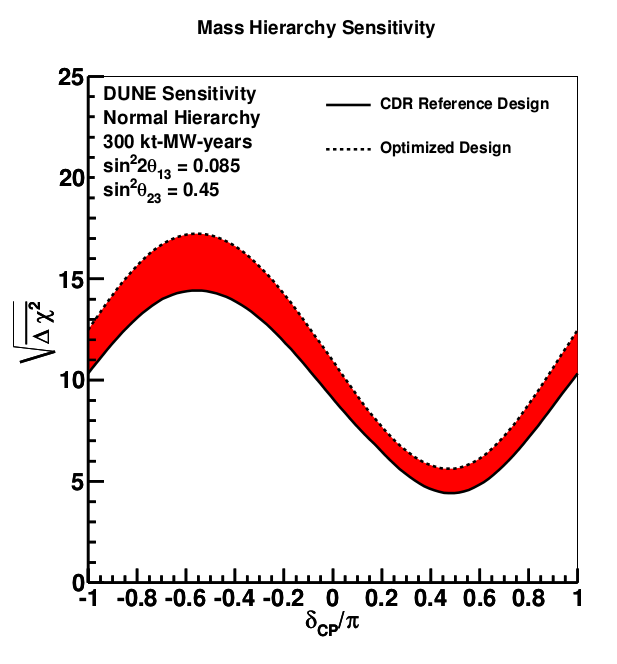
\includegraphics[width=0.30\textwidth, keepaspectratio=true]{figs/sensitivity_MH.png}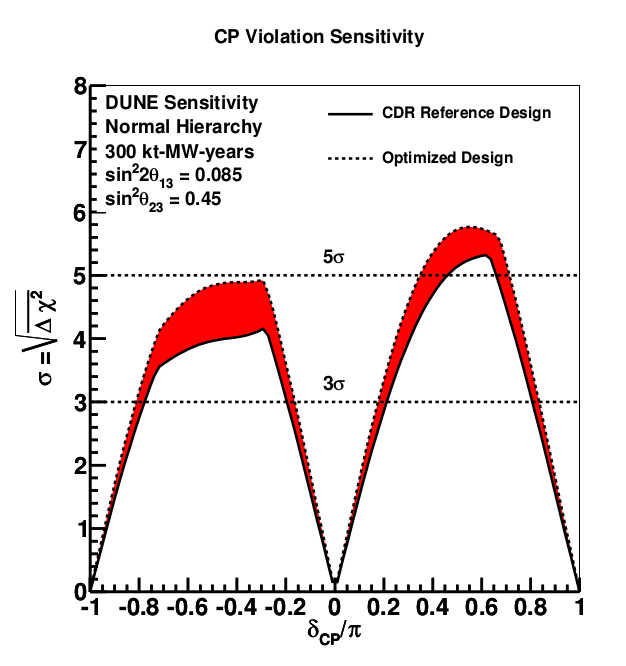
\includegraphics[width=0.31\textwidth, keepaspectratio=true]{figs/sensitivity_CP.png}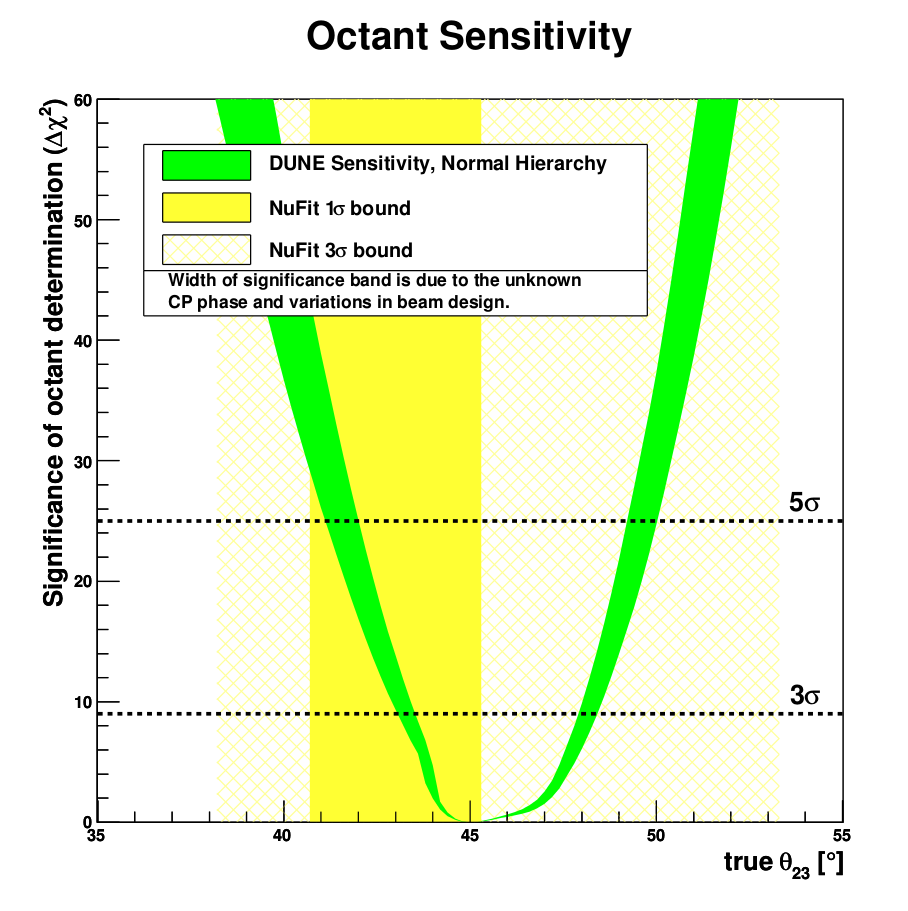
\includegraphics[width=0.32\textwidth, keepaspectratio=true]{figs/sensitivity_theta23.png}
\end{figure}
%%%%%%%%%%%%%%%%%%%%%%%%%%%%%%%%%%%%%%%%
%% if reference beam only
%%%%%%%%%%%%%%%%%%%%%%%%%%%%%%%%%%%%%%%%
%% if also has optimized beam
%\begin{table}[h]
%  \centering
%  \begin{center}
%  \caption{ The exposure needed to perform measurements with certain precision expressed in $MW \cdot kt \cdot years$. Estimates provided in the table assume normal mass hierarchy and best fit values of the known parameters }
%  \begin{tabular}{|c|c|c|}
%  \hline  
%  Physics milestone & Exposure, $MW \cdot kt \cdot years$ & Exposure, $MW \cdot kt \cdot years$ \\ \hline
%   & (reference beam) & (optimized beam) \\ \hline
%  $1^0$ $\theta_{23}$ resolution ($\theta_{23}~=~42^0$) & 70 & 45 \\ \hline
%  CPV at $3\sigma$ $(\delta_{CP}=+\pi/2)$ & 70 & 70 \\ \hline
%  CPV at $3\sigma$ $(\delta_{CP}=-\pi/2)$ & 160 & 100 \\ \hline
%  CPV at $5\sigma$ $(\delta_{CP}=+\pi/2)$ & 280 & 210 \\ \hline
%  MH at $5\sigma$ (at worst) & 400 & 230 \\ \hline
%  $10^0~\delta_{CP}$ resolution at $\delta_{CP}=0$ & 450 & 290 \\ \hline
%  CPV at $5\sigma$ $(\delta_{CP}=-\pi/2)$ & 525 & 320 \\ \hline
%  CPV at $5\sigma$, $50\%$ of $\delta_{CP}$ & 810 & 550 \\ \hline
%  CPV at $3\sigma$, $75\%$ of $\delta_{CP}$ & 1320 & 850  \hline
%  \label{tab:exposures_needed}
%  \end{tabular}
%  \end{center}
%\end{table}
